\documentclass{article}

\usepackage{graphicx}
\usepackage[utf8]{inputenc}
\usepackage[italian]{babel}
\usepackage{amsmath}

\begin{document}

\begin{titlepage}
\newcommand{\HRule}{\rule{\linewidth}{0.5mm}}
\center


\begin{figure}
\center

\includegraphics[scale=0.1]{logo}
\end{figure}


\textsc{\LARGE Università di Padova}\\[1.5cm]
\HRule \\[0.4cm]
{ \huge \bfseries Spettroscopia a prisma}\\[0.4cm]
\HRule \\[1.5cm]

\begin{minipage}{0.4\textwidth}
\begin{flushleft} \large
\emph{Autori:}\\
Raffaele \textsc{La Torre} \\
Stefano \textsc{Campostrini}
\end{flushleft}
\end{minipage}
~
\begin{minipage}{0.4\textwidth}
\begin{flushright} \large
\emph{Supervisore:} \\
Prof.ssa Caterina \textsc{Braggio}
\end{flushright}
\end{minipage}\\[4cm]

{\large \today}\\[3cm]

\vfill
\end{titlepage}

\tableofcontents

\newpage
\begin{abstract}
Lo scopo dell'esperimento consiste nel determinare l'indice di rifrazione $n(\lambda)$ del vetro di cui è costituito il prisma, dipendente dalla lunghezza d'onda della luce incidente. Come sorgente di onde elettromagnetiche è utilizzato il Cadmio che presenta cinque righe distinte, di lunghezza nota. \\
La Fig.1 mostra la deviazione e la dispersione di un raggio di luce che passa attraverso il prisma. 

\begin{figure}[!ht]
\center
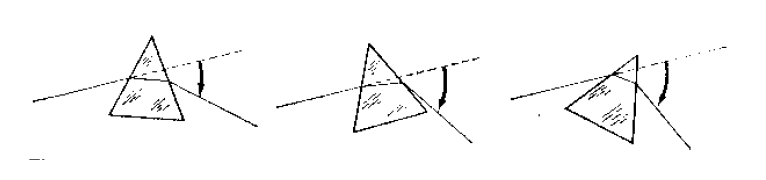
\includegraphics[scale=0.5]{prisma2}
\caption{Deviazione e dispersione di un raggio di luce che passa attraverso il prisma}
\end{figure}

L'angolo di deviazione della luce varia a seconda dell'inclinazione del prisma, e raggiunge un valore minimo che indichiamo con $\delta_{min}$, che si verifica quando il fascio rifratto sulla prima superficie è parallelo alla base. \\
Si può dimostrare che l'indice di rifrazione del mezzo prismatico è dato dalla seguente equazione: 

\begin{equation}
n = \frac{\sin(\frac{\alpha + \delta_{min}}{2})}{\sin(\frac{\alpha}{2})}
\end{equation}

dove $\alpha$ è l'angolo del vertice del prisma (quello il cui lato opposto è parallelo al primo fascio rifratto).
\end{abstract}

\newpage
\section{Apparato Sperimentale}
L'apparato sperimentale consiste in uno spettroscopio, schematizzato in Fig.2. \\
Una struttura cilindrica supporta un tavolo rotante coassiale che porta il prisma. Dal supporto si protendono due bracci: uno viene fissato rigidamente al supporto e porta un collimatore con una fenditura di apertura variabile; sul secondo braccio è montato un telescopio che riceve la luce dal prisma. Il ramo su cui è montato il telescopio può ruotare indipendentemente attorno all`asse centrale, per la ricerca di una particolare componente spettrale, e porta una scala graduata (interna) che si muove rispetto ad una scala graduata esterna. Sono presenti due zone sulla scala graduata, diametralmente opposte, che permettono di effettuare la misura; questo per limitare gli errori dovuti all'eccentricità.

\begin{figure}[!ht]
\center
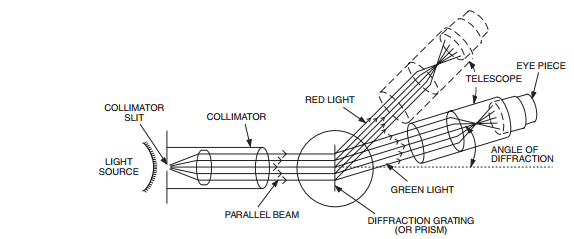
\includegraphics[scale=0.8]{spettroscopio2}
\caption{Schematizzazione dello spettroscopio}
\end{figure}

Le lunghezze d'onda del Cadmio sono note, e sono riassunte in Tab.1.

\begin{table}[h]
 \center
 \begin{tabular}{|c|c|}
   \hline
   $\lambda$ $(nm)$ & colore \\ \hline
   441.6 & violetto \\
   467.8 & blu \\
   480.0 & azzurro \\
   508.6 & verde \\
   643.8 & rosso \\ \hline
 \end{tabular}
 \caption{Lunghezze d`onda delle righe spettrali del Cadmio}
\end{table}

L'errore sistematico sulla lettura dell'angolo è $\Delta\theta = 0^{\circ} 02'$.

\newpage
\section{Procedura}
La procedura è divisa nelle seguenti fasi:

\begin{enumerate}
\item Determinare l'angolo di deviazione minima $\delta_{min}$. 
  \begin{enumerate}
  \item La misura dell’angolo di deviazione minima avviene cercando inizialmente attraverso l’oculare del  cannocchiale il raggio rifratto dal prisma. A questo punto si insegue il raggio sempre verso la direzione del fascio di luce incidente con il cannocchiale ruotando nello stesso verso la piattaforma di sostegno del prisma. La  configurazione di angolo $\theta_{min}$ in cui l’immagine inverte il senso del suo spostamento corrisponde alla configurazione di minima deviazione.
  \item Misurare l'angolo $\theta_0$ del fascio indeflesso.
  \item L'angolo $\delta_{min}$ cercato è dato da $\delta_{min} = \theta_0 - \theta_{min}$
  \end{enumerate}
\item Determinare l'angolo al vertice $\alpha$. La Fig.3 è riferita alla configurazione di minima deviazione.
  \begin{enumerate}
  \item Facendo riferimento alla Fig.3, porre il prisma nella condizione di minima deviazione.
  \item Misurare l'angolo di riflessione $\theta_r$ sulla scala graduata.
  \item Dal valore di $\theta_r$ e $\delta_{min}$ si può ricavare il valore di $\alpha$ (vedere la sezione "Elaborazione dati").
  \end{enumerate}              
\end{enumerate}

IMMAGINE 3 (DA FARE)

\newpage
\section{Raccolta dati}
Tutte le misure raccolte in parentesi quadre indicano la lettura dell'angolo riferita al secondo nonio, per correggere l'errore dovuto all'eccentricità del supporto girevole su cui è collocata la scala graduata. \\
La Tab.2 riassume le misure effettuate per le cinque lunghezze d'onda per determinare $\delta_{min}$.

\begin{table}[h]
 \center
 \begin{tabular}{|c|c|c|c|}
   \hline
   $\lambda$ $(nm)$ & $\theta_0$ & $\theta_{min}$ & $\delta_{min}$ \\ \hline
   441.6 & $330^{\circ} 52'$ & $291^{\circ} 16'$ & $39^{\circ} 34'$ \\
         & [$150^{\circ} 50'$] & [$111^{\circ} 20'$] & [$39^{\circ} 30'$] \\ \hline
   467.8 & $330^{\circ} 50'$ & $291^{\circ} 30'$ & $39^{\circ} 20'$ \\ 
         & [$150^{\circ} 50'$] & [$111^{\circ} 34'$ & [$39^{\circ} 16'$] \\ \hline
   480.0 & $330^{\circ} 52'$ & $291^{\circ} 38'$ & $39^{\circ} 14'$ \\ 
         & [$150^{\circ} 52'$] & [$111^{\circ} 42'$ & [$39^{\circ} 10'$] \\ \hline
   508.6 & $330^{\circ} 40'$ & $291^{\circ} 38'$ & $39^{\circ} 02'$ \\ 
         & [$150^{\circ} 40'$] & [$111^{\circ} 40'$ & [$39^{\circ} 00'$] \\ \hline
   643.8 & $330^{\circ} 44'$ & $292^{\circ} 14'$ & $38^{\circ} 30'$ \\ 
         & [$150^{\circ} 42'$] & [$112^{\circ} 18'$ & [$38^{\circ} 24'$] \\ \hline
 \end{tabular}
 \caption{Angoli misurati per le cinque lunghezze d'onda delle righe spettrali del Cadmio}
\end{table}

Si elencano ora i due valori di $theta_r$ misurati, relativamente alle lunghezze d'onda del blu e del verde: \\
\begin{center}
$\theta_{r_1} = 51^{\circ} 00' $ \\
$[\theta_{r_1} = 230^{\circ} 54']$ \\
$\theta_{r_2} = 51^{\circ} 10'$ \\
$[\theta_{r_2} = 231^{\circ} 04']$ 
\end{center}


\newpage
\section{Elaborazione dati}


\newpage
\section{Conclusioni}

\end{document}
